\documentclass[xcolor=dvipsnames, 12pt]{beamer}

\usepackage{appendixnumberbeamer}
\usepackage{graphicx}
%\usepackage{url}
\usepackage[english]{babel}
\usepackage[utf8]{inputenc}
\usepackage[T1]{fontenc}
\usepackage{marvosym}
\usepackage{ulem}
\usepackage{listings}
\usepackage{units}

\setbeamertemplate{navigation symbols}{}

\mode<presentation>
{
  \usetheme{Madrid}
  \usefonttheme[onlylarge]{structuresmallcapsserif}
  \usefonttheme[onlysmall]{structurebold}
  \setbeamerfont{frametitle}{size=\large}
  \setbeamerfont{title}{size=\large}
  \setbeamerfont{section in toc}{size=\normalsize}
  \setbeamercovered{invisible}
}

\definecolor{UniManPurple}{rgb}{0.31,0.,0.49}
\definecolor{UniManYellow}{rgb}{1.,0.85,0.}
\usecolortheme[rgb={0.31,0.,0.49}]{structure}              % UM colorf
\newcommand{\MYTITLECOLOUR} {\textcolor[rgb]{1.,0.85,0.}}  % UM yellow
\newcommand{\PURPLE} {\textcolor[rgb]{0.31,0.,0.49}}  % UM purple
\newcommand{\BF}[1]{\begin{frame}{\MYTITLECOLOUR{#1}}}  % UM yellow
\definecolor{silver}{gray}{0.61}

\lstset{ %
  captionpos=n,
  language=Python,
  basicstyle=\tt
}

\newenvironment{myFrame}[1]%
{\begin{frame}{\MYTITLECOLOUR{#1}}}%
{\end{frame}}

\AtBeginSection[]
{
  \begin{myFrame}{Outline}
  \tableofcontents[currentsection, currentsubsection, hideothersubsections]
  \end{myFrame}
}

% http://tex.stackexchange.com/questions/67064/a-thicker-wave-underline
\catcode`\@=11 %
\font\uwavefont=lasyb10 scaled 652
\def\uwave{%
  \bgroup
    \markoverwith{%
      \lower3.5\p@\hbox{\uwavefont\char58}%
    }%
  \ULon
}

\begin{document}


\hypersetup{
  hidelinks=false,
  colorlinks=true,
  linkcolor=blue,
  urlcolor=blue,
  citecolor=blue,
  anchorcolor=blue
}
\makeatletter
\Hy@colorlinkstrue
\Hy@ocgcolorlinkstrue
\Hy@frenchlinkstrue
\def\Hy@colorlink#1{%
  \begingroup
  \HyColor@UseColor#1%
}%
\def\Hy@endcolorlink{\endgroup}%
%\def\@pdfborder{0 0 0.5 [3 3]}%
%\let\@pdfborderstyle S
\makeatother



%\title[\MYTITLECOLOUR{Programming}]{\MYTITLECOLOUR{Programming with Python}}
\title{\MYTITLECOLOUR{Programming with Python}}

\author[V. \v{S}ego]{
\textbf{\PURPLE{Vedran \v{S}ego}} {\tt <\href{mailto:vsego@vsego.org}{vsego@vsego.org}>}
}
\date{29.1.2015.}

\titlegraphic{
\includegraphics[width=2.7cm]{manchesterlogo}\hspace*{4.75cm}~%
   
\includegraphics[height=1cm]{nalogo}}

\begin{frame}[plain]
%\titlepage
  \centering
  \setbeamercolor{block body}{bg=UniManPurple,fg=UniManYellow}
  \begin{block}{}\centering
    \vskip3mm
    \usebeamerfont{title}\inserttitle\par
    \vspace*{4mm}
  \end{block}
  \usebeamerfont{author}\insertauthor\par
  \usebeamerfont{institute}\insertinstitute\par
  \usebeamerfont{date}\insertdate\vskip-4mm
  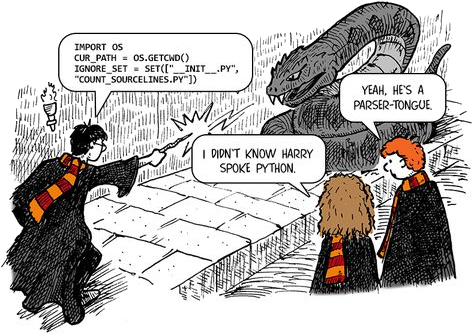
\includegraphics[height=.6\textheight]{images/ForallyoucodersHarryspeakspython-32556.png}\par
  \usebeamercolor[fg]{titlegraphic}\inserttitlegraphic
\end{frame}

\begin{myFrame}{Outline}
\tableofcontents[hideothersubsections]
\end{myFrame}

\section{Basics}

\subsection{The course and the lecturer}

\begin{myFrame}{Who? What? Where?}
\vskip-2mm\hfill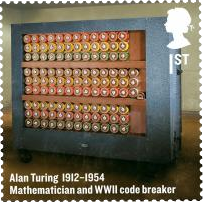
\includegraphics[height=29mm]{images/stamp.png}\vskip-19mm
\begin{itemize}
  \item Name: Vedran \v{S}ego
  \item Office: 1.218
  \item E-mail: \href{mailto:vsego@vsego.org}{\texttt{vsego@vsego.org}} \par
    Please use:
    \begin{itemize}
      \item only \alert{plain text} (no HTML nor non-standard characters),
      \item \alert{clear, informative subjects}.
    \end{itemize}
  \item Office hours: Friday, 12:00--13:00
  \item The course website:\par
    \href{http://vsego.org/math20622}{http://vsego.org/math20622} or \href{http://vsego.org/math20622}{http://vsego.org/python}
\end{itemize}
\end{myFrame}



\section{Aims of the course}

\subsection{Where does this course stand}

\begin{myFrame}{Where can I use any of this?}
While we shall cover none of these topic, you should become able to ``dig out'' on your own how to tackle the problems in:
\begin{enumerate}
  \item Matrix Analysis (MATH36001) -- SciPy and NumPy modules;
  \item Combinatorics and Graph Theory (MATH39001) -- modules {\tt math}, {\tt itertools}, {\tt combinatorics}, {\tt pyncomb}, {\tt qombinatorics}, {\tt networkx}, built-in lists and dictionaries (see \href{http://www.python-course.eu/graphs_python.php}{here});
  \item Mathematical Biology (MATH35032) -- {\tt SciPy} module for ODEs, {\tt PyMOOSE} module, built-in lists and dictionaries;
  \item Problem Solving by Computer (MATH36032) -- Python and MATLAB are quite similar (and somewhat a competition);
  \item Mathematical Programming (MATH39012) -- modules {\tt PyLPSolve}, {\tt CVXOpt}, {\tt PyGLPK}, {\tt PyMathProg}.
\end{enumerate}
And these are just some of the $3^\text{rd}$ year undergraduate courses.
\end{myFrame}

\begin{myFrame}{In this course\dots}
\dots{}we aim to learn how to:
\begin{enumerate}
  \item analyze a problem,
  \item construct an algorithm that solves it,
  \item write a program that implements the said algorithm.
\end{enumerate}\vskip2ex
\onslide<2->
Be careful!
\begin{itemize}
  \item Where do I expect ``\alert{trouble}''? \par
    Point 2: the so called {\itshape algorithmic way of thinking}. \par
\onslide<3->
  \item Why? \par
    This is \alert{fundamentally new} to those with no experience with programming.
\end{itemize}\vskip2ex
\onslide<4->{
{\bfseries Our language of choice:} Python 3 {\small (with some effort, fairly simple!)}
}
\end{myFrame}

\begin{myFrame}{However,\dots}
\dots{}we do \alert{{\bfseries not} aim} to:
\begin{itemize}
  \item make you into World class programmers (this would take at least a whole programme and does not fit in a single course),
  \item address all the features and the libraries of Python (this would take even longer),
  \item learn ``dark'' tricks that almost all languages have.
\end{itemize}\vskip3ex
\onslide<2->
\alert{\bfseries Our aim} is ``only'' to lay a strong foundation for your future programming requirements, be they in Python or some other language or a similar tool.\vskip3ex
\onslide<3->
Don't worry, this is \alert{not as easy as it sounds}. \Smiley{}
\end{myFrame}

\subsection{A note on the language}

\begin{myFrame}{Father and son}
Python currently has two branches:
\begin{itemize}
  \item Python 2: old(-ish), well established, widely used;
  \item Python 3 (\alert{our choice}): newer, better designed, also widely used, gaining acceptance, some modules are not converted (yet), but almost all widely used either are converted or will soon be.
\end{itemize}\vskip2ex
The two are very similar, but there are some significant differences! \par
\hskip7mm $\Rightarrow$ Some of these will be addressed as necessary. \vskip2ex
\onslide<2->
Our focus is on \alert{algorithms}, not on the programming language! \par
\hskip7mm $\Rightarrow$ Python specifics will be avoided as much as possible. \par
\hskip7mm \phantom{$\Rightarrow$} {\small (but they will be shown for those interested in Python itself)}
\end{myFrame}

\subsection{Lectures and lab classes}

\begin{myFrame}{Lectures and lab classes}
\begin{itemize}
  \item Week 1:
    \begin{itemize}
      \item This lecture: about the course.
      \item Lab class (tomorrow): the first lecture.
    \end{itemize}
  \item From the second week on:
    \begin{itemize}
      \item Lectures: covering the new material.
      \item Lab class: students solve problems on computers.
    \end{itemize}
\end{itemize}
\end{myFrame}

\subsection{Marking}

\begin{myFrame}{Marking}
\begin{itemize}
  \item Six one-hour tests during the lab classes (30\%):
    \begin{itemize}
      \item The \alert{best five} will be taken into account.
      \item The first one is in week 3.
      \item Two problems on each; 3 points per problem.
      \item Small(-ish) programs done on computers.
      \item Covering the material up to the previous week.
    \end{itemize}
  \item Coursework at the end of semester (70\%):
    \begin{itemize}
      \item A project to program at home.
    \end{itemize}
\end{itemize}
\end{myFrame}



\section{How to tackle this course}

\begin{myFrame}{How to tackle this course?}
\begin{center}
{\itshape Programming is a skill. It cannot be learnt; it has to be crafted.}\par
\hfill --- prof.\ Saša Singer, University of Zagreb
\end{center}
\onslide<2->
This means:
\begin{itemize}
  \item Traditional ``learning by reading'' is of \alert{little use}.
  \item Trial-and-error \alert{on a computer} is the only way to learn!
  \item Programming cannot be learnt the night (or even a day or two) before the exam!
\end{itemize}
\onslide<3->
Why?
\begin{itemize}
  \item Remember the ``fundamentally different algorithmic way of thinking'' from a few slides before?
  \item Too many details to consider -- \alert{\bfseries experience is crucial!} \par
    (and you're here to get some of it)
\end{itemize}
\vskip2ex
\end{myFrame}

\begin{frame}[fragile]{\MYTITLECOLOUR{How to actually do this? (1)}}
\begin{itemize}
  \item \alert{Copy/paste} (from the ready made examples and solutions) \alert{is {\bfseries not} your friend!} If you must use such a solution, \alert{retype} it, so you notice the important details! \par
  \onslide<2->
  For example, these four are \alert{different types} of data, mostly with \alert{very different properties}:\vskip-2mm
  {\small \begin{lstlisting}
    f = ( "x", 17, "y", 19, "z", 23 )
    b = [ "x", 17, "y", 19, "z", 23 ]
    r = { "x", 17, "y", 19, "z", 23 }
    j = { "x": 17, "y": 19, "z": 23 }
  \end{lstlisting}}
  Will you notice and remember the type of brackets or which of the comma/colon was used if you just copy/paste a program with only \alert{one} of these? \par
  \onslide<3->
  How about the difference between these two?\vskip-2mm
  {\small \begin{lstlisting}
    f = h
    g = h(x)
  \end{lstlisting}}
\end{itemize}
\end{frame}

\begin{myFrame}{How to actually do this? (2)}
\begin{itemize}
  \item Using a solution from a lecture or some other source is fine a \alert{first few times} when you encounter a new subject, but even then do \alert{\bfseries NOT} just retype.\par
    Run the program and \alert{test it} (give it some input and check that the output is correct). \par
\onslide<2->
    Take a break from it and, some hours later, \alert{try to write your own solution} to the same problem, without looking at or trying to recall the ``official'' solution.
\onslide<3->
  \item \alert{\bfseries Do NOT learn chunks of code by heart!} \par
    These cannot be just ``reused''; \alert{they must be {\bfseries understood}!} \par
    Otherwise, you get a wrong impression of ``understanding'', which \alert{backfires} in exams and practical situations.
\end{itemize}
\end{myFrame}

\begin{myFrame}{How to actually do this? (3)}{}
{\large\bfseries Write programs on your own!}
\onslide<2->
\begin{itemize}
  \item \alert{Read the errors and warnings} that Python writes out. \par
    These are crucial to understand what went wrong!
\onslide<3->
  \item As before, \alert{test your program!} Run it several times, give it some input, and \alert{check the results}! \par
    % An example: where does a plane go? To Birmingham... UK or Alabama?
    If they are wrong, read your code and try to figure which part(s) produce a result different from what you expected.
\onslide<4->
  \item Test the \alert{boundary cases}! \par
    Does your expansion to prime factors work if the input itself is a prime number? What if it's a negative number? \par
    Does your algorithm work properly with the first/last member of the list, or only with the ones in the middle? How about an empty list? \par
    \dots
\end{itemize}
\end{myFrame}

\begin{myFrame}{How to actually do this? (4)}{}
What if it doesn't work out?
\onslide<2->
\begin{enumerate}
  \setcounter{enumi}{-1}
  \item Try until you run out of ideas.
  \item If you cannot make the program work as it should, read the solution and \alert{analyze it}. Try to figure out how it works, how it was constructed, and why your own didn't work.
  \item Then return to it later and try to solve the problem without using the solution (reading Python documentation is always fine).
  \item If that fails, go back to step 1.
  \item If you have to do this for (almost) all problems, seek help with the staff. \alert{Do not wait for the exams} to address the issue! \par
    \alert{This process takes time and effort!}
\end{enumerate}
\onslide<3->{
{\bfseries Remember:} Your solution need not be the same as the ``official'' one, but it has to produce the correct results.

(Almost) all problems have many (more or less different) solutions.\vskip1ex
}
\onslide<4->
By the way, the above is an example of an algorithm. \Smiley{}
\end{myFrame}

\begin{myFrame}{How to actually do this? ($9\,\unitfrac{3}{4}$)}
\begin{center}
How you approach these classes might also have a wee bit of an impact on the whole "crafting your programming skills" process... \Smiley{} \vskip.7ex
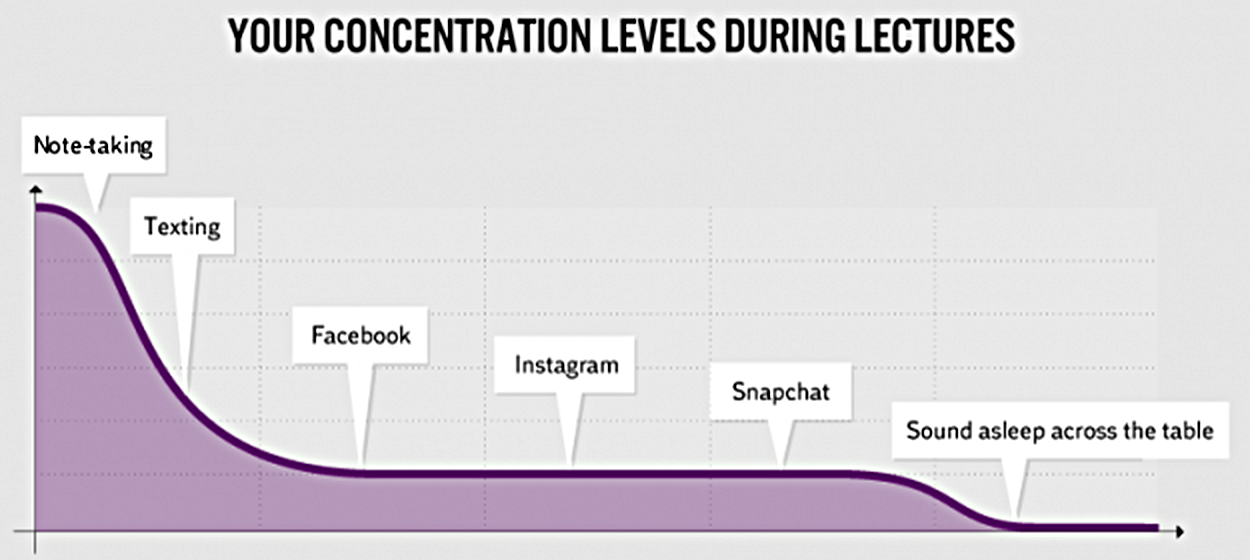
\includegraphics[width=.87\paperwidth]{images/concentration-levels.png} \vskip-.7ex
{\tiny [\href{http://kindofnormal.com/truthfacts/2015/01/27}{Image source}]}
\end{center}
\end{myFrame}



\section{Some final remarks}

\subsection{Asking for help}

\begin{myFrame}{Asking for help (1)}
If you encounter a problem, address it immediately -- \alert{most of the lectures rely on the \uwave{understanding} of the previous ones!} \par
\begin{columns}[T]
\begin{column}{0.96\textwidth}
You can ask:
\begin{itemize}
  \item teaching assistants,
  \item me,
  \item your colleagues (be careful, though),
  \item on-line. \par
    I suggest \href{http://stackoverflow.com/}{Stack Overflow}. Before asking a question there, \alert{read their instructions!} The community is very helpful, but they require effort and will not just solve your problems for you.
\end{itemize}
\end{column}
\begin{column}{0pt}
\vspace*{2mm}\hskip-19mm
\includegraphics[width=19mm]{images/keep-calm-and-ask-for-help.png}
\end{column}
\end{columns}
\end{myFrame}

\begin{myFrame}{Asking for help (2)}
At a more advanced level:
\begin{itemize}
  \item \href{http://codereview.stackexchange.com/}{Code Review Stack Exchange} -- get expert opinion and advice on your \alert{properly working} code;
  \item \href{http://programmers.stackexchange.com/}{Programmers Stack Exchange} -- for conceptual questions about software development.
\end{itemize}
As before, \alert{read their instructions before asking a question!}\vskip2ex
\onslide<2->{
{\bfseries Hint:} There is also \href{http://math.stackexchange.com/}{Mathematics Stack Exchange}\dots 
}
\end{myFrame}

\subsection{Useful references}

\begin{frame}[fragile]{\MYTITLECOLOUR{References (1)}}
Some useful references:
\begin{itemize}
  \item For most of the questions, it is enough to Google \par
    {\tt python3 whatever you want to know}
  \item The official \href{https://docs.python.org/}{Python 3 documentation} (there is also a \href{https://docs.python.org/2.7/}{Python 2 documentation}, if you ever need it),
  \item Built-in help, invoked from Python itself:
    \begin{lstlisting}
    help(print)
    \end{lstlisting}
    or
    \begin{lstlisting}
    import numpy
    help(numpy)
    \end{lstlisting}
  \item Aforementioned Stack Exchange sites.
\end{itemize}
\end{frame}


\begin{myFrame}{References (2)}
\begin{center}
\vskip-5mm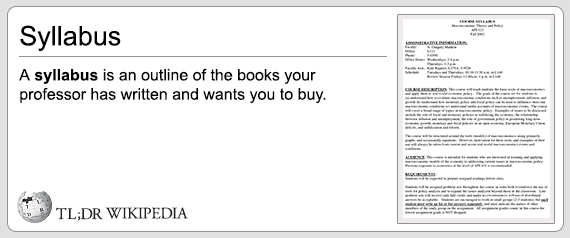
\includegraphics[width=83mm]{images/syllabus.png}
\end{center}\vskip-3mm
For those preferring dead wood books,
\begin{itemize}
  \item Mark Lutz, ``Learning Python''. (no, I am not Mark Lutz \Smiley{})
\end{itemize}
For those already familiar with programming, just not in Python:
\begin{itemize}
  \item Mark Pilgrim, ``\href{http://www.diveintopython3.net/}{Dive into Python 3}'' (freely downloadable HTML and PDF); you can also buy a dead wood version, or install it for free on Android devices. \par
    There is a \href{http://www.diveintopython.net/}{Python 2 version} as well.
\end{itemize}
\end{myFrame}

\begin{frame}[fragile]{\MYTITLECOLOUR{Homework}}
\begin{itemize}
  \item Install Python 3 (the instructions are on the course web site) on your home computer.
  \item Try running this program to verify that your Python installation works properly:
    \begin{lstlisting}
    import this
    \end{lstlisting}
    Yes, there is only one line and there are no interpunctions. \par
    It should print a poem ``The Zen of Python'', by Tim Peters.
    \onslide<2->
    And yes, there is some weird humor in Python. After all, it was named after (somewhat famous) Monty Python. \par
    \onslide<3->
    But don't worry, none of it affects ``real'' programming\dots
\end{itemize}
\end{frame}

\begin{frame}[plain]
\begin{center}
{\large That's all for today (unless, of course, there are questions)}\vskip.17ex
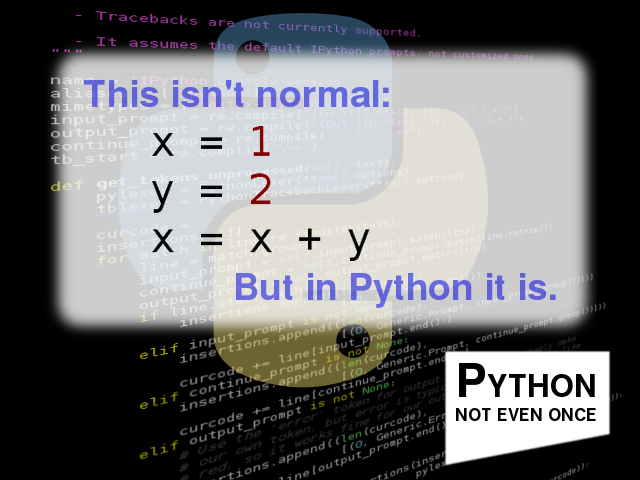
\includegraphics[height=.5\textheight]{not-even-once/not-even-once.png}\vskip.17ex
{\bfseries\LARGE Thank you for your attention!}
\end{center}
\end{frame}



\end{document}
